\documentclass[a4paper,twocolumn]{article}

\usepackage[utf8]{inputenc}
\usepackage[T1]{fontenc}
\usepackage{textcomp}

\usepackage{amsmath}
\usepackage{amssymb}
\usepackage{graphicx}

\title{Style Based Drawn Artwork Image Classification}
\author{Michal Grochmal
  $<$\href{mailto:grochmal@member.fsf.org}{grochmal@member.fsf.org}$>$
}
\date{\today}

\usepackage[colorlinks=true]{hyperref}

\hyphenation{ge-ne-ric Ge-ne-ric Ro-me-ro Ma-ria}

\begin{document}
\maketitle

\section{Introduction}

Content Based Information Retrieval systems for images or simply Content Based
Image Retrieval systems (CBIR systems) retrieve images from large collections
similar to a query image.  Yet, what \emph{"similar"} means in this context
varies;  similarity depends on the nature of the collection and on what
\emph{meaning} (semantics) contained in the query image we want to search for.
A specific query image may contain more than one meaning.  e.g. we might query
a collection of personal photos using a picture of our cousin holding a
carnival mask in Venice.  For this query image we might want to ask: whether
there are photos of our cousin in the collection, or whether there are photos
of venetian carnival masks, or photos with a specific building or location in
Venice in the background.

Each type of collection of images needs a different \emph{set of features} that
allows searching for similar images within a semantic context.  This work will
evaluate features for CBIR in the retrieval of art images in the contexts of
similar style of illustrations, drawings and paintings.  \emph{Aesthetics} are
deeply related to the concept of art \cite{rmc12ajs} therefore similar style
will be discussed by the evaluation of aesthetics of the images, whilst
ignoring the content of the image.  Back to the example of the query image with
our cousin holding a carnival mask in Venice we would try to evaluate the
quality of the framing of the photo, and ignore the presence of our cousin, the
mask and the location.

Although completely ignoring the content of an image is probably impossible,
features that are independent of the objects in the image exist.  Such features
are more relevant in works of art \cite{zirnhelt07art} as the meaning of how
objects are drawn is important for how humans see a piece of art
\cite{mach10clas}.  In this work, we will use \emph{aesthetic features} tried
on collections of drawn artwork (illustration, drawing and painting) and on
collections of photography, and apply them for classification of artwork with
the meaning of identifying the author of the artwork.  Further, we will try to
extrapolate the meaning of these features and try to identify images of the
same art school and same art period.

\begin{figure}[!htb]
\centering
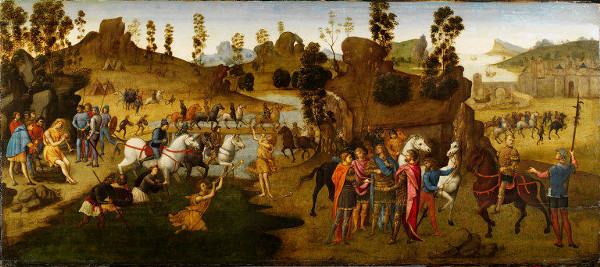
\includegraphics[width=0.48\textwidth]{diff_caesar}
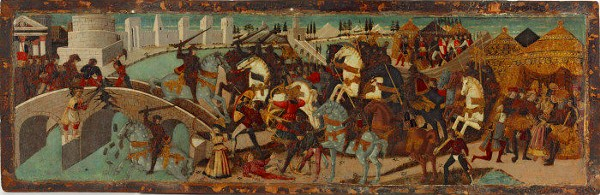
\includegraphics[width=0.48\textwidth]{diff_horatius}
\caption{The image at the top is the painting "Julius Caesar and the Crossing
of the Rubicon" by Francesco Granacci and at the bottom is the panel "Horatius
Cocles Defending the Sublician Bridge" by Francesco Pesellino.  Both images
have a similar theme and the objects contained in them are similar, yet the
style of the images is different.}
\label{diff}
\end{figure}

\begin{figure}[!htb]
\centering
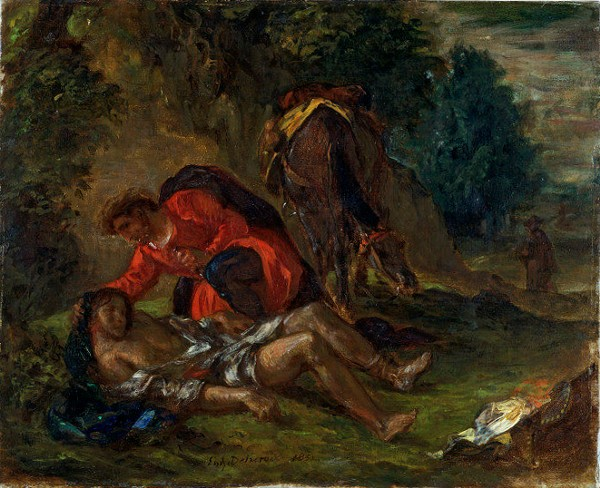
\includegraphics[width=0.48\textwidth]{sim_delacroix_samaritan}
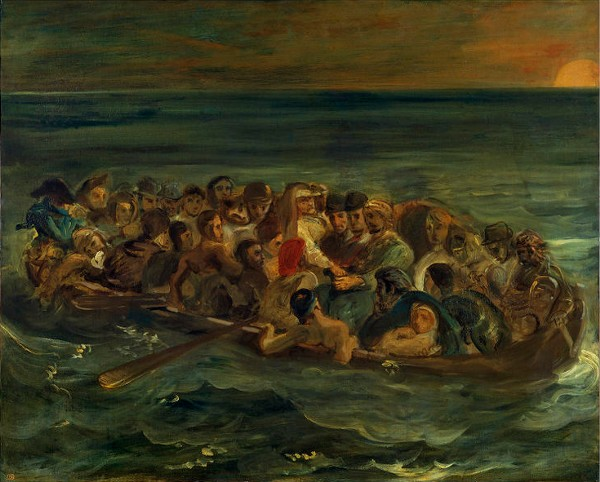
\includegraphics[width=0.48\textwidth]{sim_delacroix_shipwreck}
\caption{In these two paintings by Delacroix, "The Good Samaritan" and "The
Shipwreck of Don Juan", we can see a similar style.  Both paintings are
different in their theme, yet the author's style of drawing and paining can be
easily noticed by humans.}
\label{similar}
\end{figure}

Figures \ref{diff} and \ref{similar} shows an example of similarity by style.
In Figure \ref{diff} we see paintings by Francesco Granacci and by Francesco
Pesellino which are closely related by context and objects present, both
paintings represent military actions of the Roman Empire.  Yet the style of
these two images is different.  Figure \ref{similar} shows two paintings by
Delacroix, these paintings show two different scenes yet their \emph{style is
similar}.  The style of an image caries the signature of it's creator and the
art movement the creator was part of.  [All images are from the public
collection of the Victoria and Albert Museum in London, this collection will be
used as a dataset in this work.  Se section \ref{datasets} for more information
about this collection.]

The classification of images by style is needed for CBIR systems for artwork
\cite{cfsp12air,isv12mpeg}, and a better understanding of the features needed
for this classification will help in the further development of such systems.
Big collections of artwork, e.g. collections maintained by museums and
galleries, would also benefit from better classification techniques: Often
items in these collections have incomplete or \emph{missing metadata}, finding
which other collection items are similar to these items will allow a computer
to fill the missing metadata automatically.  Finally, an algorithm that
understands style in art understands more than just the content of images.  As
discussed in \cite{rmc12ajs}, such algorithm leads us closer to computers that
can understand art, and creativity.

\section{Related Work}

Production CBIR systems for art, two of which are described in \cite{cfsp12air}
and in \cite{ymvz03tree}, use colour, colour disposition and texture as
features to retrieve drawings, illustrations and/or paintings.  These features
capture the style of the image better than corner detection or interest points
(as in SIFT or MSER) used in object recognition and duplicate detection
\cite{szel11book}, as the later describes the content of the image.

On research ground, works explore richer sets of features, yet these works
focus on photography rather than drawn art.  Estimates of \emph{image
complexity} based on lossy compression errors, \emph{standard deviation} and
\emph{average} over components of \emph{HSV} representation are used by Romeo
and Correia in \cite{jma12clas,cmrc13fs,rmc12ajs}.  Itten colour harmony over
components of the \emph{HSL} representation and line estimates drawn from edges
detected in the image are used in \cite{mach10clas}.  On black and white
images, e.g.  drawings, the pioneer work by Kr\"oner \cite{kroner98draw} used
histograms of black and white over image regions instead of colour histograms.
All these features are added to colour and texture to produce features for
image classification.  Ivanova \cite{isv12mpeg} uses MPEG-7 descriptors as
features, yet MPEG-7 descriptors are just the same features encoded in a
different way.  The used MPEG-7 features are: colour histograms, colour
distribution, dominant colour, edge histogram, and texture.  We can argue that
the features explored among all these works are consistent.

A closely related field to CBIR in art is Affective Image Retrieval (AIR)
summed by Machajdik in \cite{mach10ua,mach10clas}.  In this field both the
style and the content of the image is important, yet it is important that the
style and the content are separately evaluated.  In the project at hand we are
not interested in the content of the images, but the features used in AIR to
capture the style of the image may prove useful.  In AIR, features from art
theory based on Itten colours can classify an image into emotions.  \emph{Itten
colours} define colour harmony, colour warmth, completeness of contrast, hue
spread, hue count and dominant colour areas in mathematical terms which make
them image features that are simple to compute.

All features above are \emph{scale dependent} \cite{rmc12ajs,mach10clas}
therefore normalisation of the size and colour space of the image must be
performed.  The HSV/HSL colour spaces are used instead of RGB because features
extracted from those colour spaces can be linked to human perception.  Even
better, we can link a feature extracted from only one component of HSV or HSL
to human perception (e.g. how bright the image is), this is not possible in the
RGB colour space \cite{rmc12ajs}.

The major datasets used in \cite{rmc12ajs,mach10clas} are of photography
(because of the wide availability of such datasets) therefore some of the
features have not yet been tried on drawn art.  Just small datasets of art were
tried in \cite{mach10clas} and in \cite{rmc12ajs} a task of \emph{author
identification} was partially accomplished.  A bigger dataset of drawn art was
tried in \cite{zirnhelt07art} but using a very limited set of features.
Eventually, based on the features used in the author identification a task of
artistic period and art school identification is proposed in
\cite{zirnhelt07art} and \cite{rmc12ajs}.  In this work, we plan to fill the
gap by applying the not yet tried features to datasets of drawn art images.

% old version
%In this work, we plan to fill the gap by applying the features that have not
%yet been tried on drawn art to datasets of drawn art images.

\section{Proposed Approach}

Although it is not possible to fully separate the content of the image from
it's style, there are good approximations by using features general to the
image.  We will reproduce the features used by Romeo in \cite{rmc12ajs} and by
Machajdik in \cite{mach10clas} and apply these features to the task of author,
period and art school classification.  To perform this task we will need
software for \emph{programmatic image processing} and for classification tasks.

We will use OpenCV\footnote{available at \href{http://opencv.org/}{opencv.org}
under the BSD license} which is a library that provides a big set of functions
to extract features from images, and it is well integrated with many
programming languages.  For example, with OpenCV we can extract the Gray Level
Co-occurrence Matrix (GLCM) for the texture features, as it provides the needed
functions.  JPEG and fractal compression ratios will be extracted with the
ImageMagick\footnote{available at
\href{http://www.imagemagick.org/}{www.imagemagick.org} under the Apache 2.0
license} and the FIASCO\footnote{available at
\href{http://github.com/l-tamas/Fiasco/}{github.com/l-tamas/Fiasco} under the
GPLv2 license} set of command line tools, respectively.  The python imaging
library (PIL)\footnote{available at
\href{http://pythonware.com/products/pil/}{pythonware.com/products/pil} under a
generic open source license} (or it's fork Pillow) can be used as described by
Solem in \cite{solem12book} to extract colour histograms, and will also be used
to extract the features based on Itten colours.  The most complex image
transformations for feature extraction will be the Sobel and Canny filters for
edge detection, these techniques are available from OpenCV, and can also be
simulated with PIL and scipy \cite{oliphant06numpy}.

For the classification task \emph{Support Vector Machines} (SVMs) will be used,
as this technique was previously used for the author identification task by
Romeo in \cite{rmc12ajs}.  In Romeo's work LIBSVM\footnote{available at
\href{http://www.csie.ntu.edu.tw/~cjlin/libsvm/}
{www.csie.ntu.edu.tw/\~{}cjlin/libsvm} under a generic open source license} was
used, therefore we will start with that tool.  LIBSVM command line tools are
very good for prototyping, as described in \cite{hcl03svm}.  To produce
visualisation of the classified images and to allow for the use of different
classification algorithms we will resort to scikit-learn\footnote{available at
\href{http://scikit-learn.org/}{scikit-learn.org} under the BSD license}.  With
scikit-learn we will try different classification algorithms, notably Nearest
Neighbours and Stochastic Gradient Descent.  This tool set shall be enough to
replicate previous experiments and to extrapolate the experiments onto new
datasets.

If the time permits or if the features prove insufficient for the
classification, we will try a different approach.  We will try to acquire new
features by learning them from the datasets with \emph{deep learning
techniques}, as summed in \cite{antes13deep}.  To learn features from the data
we will use pylearn2\footnote{available at
\href{http://deeplearning.net/software/pylearn2/}
{deeplearning.net/software/pylearn2} under the BSD license} which is an
implementation of deep learning.

\subsection{Datasets}
\label{datasets}

Comparison between works can only be achieved if the datasets used for the
classification are published for the research community \cite{mach10clas}.  And
the datasets used in \cite{mach10clas} and in \cite{jma12clas} are published.
Yet, these two datasets are mostly of photographs, whilst the artist
identification task is to be performed over drawn art.  These two datasets are
useful to test to which level the previous work can be replicated, which, then
shall be applied to new, more suitable, datasets.

Online art collections are available from galleries and museums.  One such
collection originating from the Birkbeck College\footnote{
\href{http://www.bbk.ac.uk}{bbk.ac.uk}} through the CACHe project\footnote{
\href{http://www.bbk.ac.uk/hosted/cache/}{www.bbk.ac.uk/hosted/cache}} is the
\emph{NICE paintings (NIRP)} collection.  This collection is currently
available from the Visual Arts Data Service (VADS)\footnote{
\href{http://vads.ac.uk/}{vads.ac.uk}} project, and is tagged with metadata
about the author and period of the items.  Another suitable dataset are the
collections of the \emph{Victoria and Albert Museum (VAM)}\footnote{
\href{http://www.vam.ac.uk/}{www.vam.ac.uk}}, it's vast API extensively
describes the art items in the collections.  Both NIRP and VAM collections use
the Dublin Core Metadata Initiative\footnote{
\href{http://dublincore.org/}{dublincore.org}} as a standard for the
description of the items in the collections, therefore the items from both
collections can be identified in the same way.

The NIRP collection contains nearly 8000 pre-1900 European \emph{oil paintings}
from public collections in the UK.  In the VAM collections we are interested in
two specific subsets: paintings, containing over 2000 European oil paintings;
and drawings, containing over 2000 \emph{drawings} from Europe and USA.
Unfortunately not all items in the NIRP and VAM collections have images of good
quality and many items miss some or all metadata information, which is needed
to evaluate a classification task.  Therefore, some of the items from the
collections will need to be removed before using them as datasets for
classification.

% old version
%Yet, the collections are well maintained and the items that will need to be
%removed from them to build good datasets are few.

\subsection{Evaluation}

First of all, we will need to replicate and critically evaluate the work by
Romeo in \cite{rmc12ajs}.  The major task for this replication is the
construction of the \emph{estimate of the Kolmogorov complexity} by JPEG and
fractal image compression, as described in Romeo's work. Once the replication
of the features used by Romeo is complete we will add some of the features
described by Machajdik in \cite{mach10clas}.  In the second set of features the
majority of work will be in the implementation of \emph{Itten colours}.

We will crawl the NIRP and VAM collections for illustrations, drawings and
paintings with complete metadata.  Such items would add extra complexity not
envisioned for the classification task and will be removed from the datasets.
The resulting datasets will contain only paintings, illustrations and drawings
classified by the author and period of the item.

We will extrapolate the \emph{feature extraction and classification procedure}
previously replicated to the datasets from NIRP and VAM collections.  The
author identification task will be tried on each dataset separately and
evaluated separately.  Then both datasets will be merged into one to provide a
third dataset, and the author identification task will be tried on this third
dataset.

\emph{Principal Component Analysis} (PCA) of the NIRP and VAM datasets using
the features as components will be performed.  Together with a \emph{Pearson
Correlation} (PCC) of the classes (the authors) and the features will reveal
the most significant features from the set of features used.  PCC between
features will then be performed to find groups of closely related features.  We
will then test the classification using only one feature of each of the sets of
closely related features.

Finally, if time permits, we will extrapolate the author identification task
towards \emph{art period/school identification}.  Although this task is related
to author identification the extra complexity lies in the fact that different
collections are not consistent about this classification.  As argued by
DiMaggio in \cite{dimaggio87art} classification of art cannot be unified as it
is part of the behaviour of social groups, which always changes.  Therefore,
the art period classification will need to allow an item to be classified into
many classes at once.  And this classification will use different classes
depending on the collection the it is made against.

\subsection{Testing}

Replication of Romeo's work and of features from Machajdik's work shall be
evaluated towards achieving similar performance on the same dataset.  The
performance measure used by Romeo in \cite{rmc12ajs} is the percentage of
correctly classified images for each class (or author).  The dataset from
Romeo's work is published and will be used in a classification task that shall
\emph{replicate the previous performance}.  With the addition of features from
\cite{mach10clas} the classification performance shall not deplete.  If the
performance of the classifier depletes with the new features these shall be
removed.

Author identification task over the NIRP and VAM datasets will be then
performed using the same features and measured in the same way.  Romeo's work
on author identification contained only 6 authors (Goya, Monet, Gauguin, Van
Gogh, Kandinsky and Picasso) and from a limited time period (19th and early
20th century), yet NIRP and VAM collections contain items from many more
authors and periods.  This difference may produce different results, proving
that the set of features \emph{is good or is insufficient for author
identification} in a more heterogeneous collection.

The features selected after PCA and PCC will be evaluated in new
classifications.  Using only \emph{uncorrelated features} shall provide similar
performance as with the entire set of features.  Tests shall be compared
between runs of the full feature set and the smaller set of uncorrelated
features.

\section{Work Plan}

We will start by crawling the datasets and storing miniatures of the collection
items.  The code for the crawlers shall take \emph{one week} to build.  After
the first week, the crawlers will run whilst the feature extraction code is
being developed.  \emph{Two weeks} shall be needed for the replication of
features from Romeo's work and addition of extra feature's from Machajdik's
work.  Then, another \emph{week} will be needed to run the classifiers over the
original datasets.

In the second month we will extrapolate the features over the NIRP and VAM
datasets.  By the \emph{middle of the second month} we shall know the
effectiveness of the developed features in classifying the bigger datasets.  We
then perform PCA and PCC over the features and build classifiers using the
selected features only.  We \emph{end the second month} by statistically
comparing the classifiers with full and reduced number of features.

In the \emph{first half of the third month} we rerun our experiments and
collect the tables and graphs.  If no milestone is late at this point there
shall be extra time, and we will try the proposed art school task and the
features learned from data.  Finally, the \emph{second half of the month} is
dedicated towards finishing the report.  By the half of the third month the
report shall be already structured and drafted, yet in need of many
corrections.

\section{Limitations and Future Work}

One of the most important features proposed is the colour histogram.  The
reason for this is that before the \emph{second half of the 20th century}
artists made their pigments themselves.  Yet, in the second half of the 20th
century industrialised paints standardised colours and art from this period is
harder to distinguish by colour.  Moreover, with digital enhancements to
illustrations starting from the '90s of the previous century, the entire colour
spectrum was made available to all artists making the colour an even less
important feature for this period onwards.  Classifying art from these periods
using the same features will probably render worse results, it is left for
future work the extraction and testing of features for recent drawn artwork.

Other \emph{flat art} items (flat sculpture, porcelain or some forms of modern
art) could be classified in similar fashion as illustration, drawing and
painting.  Yet, once again, the needed features would be slightly different.
For example, the colour histogram could be used as a feature for porcelain but
we would need to ensure that all items in the collection are photographed under
the same lighting conditions.  Future work on this matter could be explored.

\bibliographystyle{plain}
\bibliography{capybara}

\end{document}

